

\documentclass{ctexart} % Default font size is 12pt, it can be changed here
\ctexset{section/format = {\Large\bfseries}}
\usepackage{geometry} % Required to change the page size to A4
\geometry{a4paper} % Set the page size to be A4 as opposed to the default US Letter
\geometry{left=1.6cm,right=1.6cm,top=3.5cm,bottom=3.5cm}
%\usepacjage{subfigure}
\usepackage{graphicx} % Required for including pictures
\usepackage{amsmath}
\usepackage{amssymb,bm}
%\usepackage{abstract}
\usepackage{float} % Allows putting an [H] in \begin{figure} to specify the exact location of the figure
%\usepacjage{wrapfig} % Allows in-line images such as the example fish picture

%\linespread{1.2} % Line spacing


%\setlength\parindent{0pt} % Uncomment to remove all indentation from paragraphs
\usepackage{enumerate}
\graphicspath{{Pictures/}} % Specifies the directory where pictures are stored

 
\newtheorem{definition}{\hspace{2em}定义}[section] % 如果没有章, 只有节, 把上面的[chapter]改成[section] 
\newtheorem{theorem}[definition]{\hspace{2em}定理} 
\newtheorem{axiom}[definition]{\hspace{2em}公理} 
\newtheorem{lemma}[definition]{\hspace{2em}引理} 
\newtheorem{proposition}[definition]{\hspace{2em}命题} 
\newtheorem{corollary}[definition]{\hspace{2em}推论} 
\newtheorem{remark}{\hspace{2em}注}[section] %类似地定义其他“题头”. 这里“注”的编号与定义、定理等是分开的




\begin{document}

%----------------------------------------------------------------------------------------
%	TITLE PAGE
%----------------------------------------------------------------------------------------

\begin{titlepage}

\newcommand{\HRule}{\rule{\linewidth}{0.5mm}} % Defines a new command for the horizontal lines, change thicjness here

\center % Center everything on the page
%%\includegraphics[width=2.5cm]{Pictures/SCE.png}
%%\textsc{\LARGE University Name}\\[1.5cm] % Name of your university/college
%%\textsc{\Large Maior Heading}\\[0.5cm] % Maior heading such as course name
%%\textsc{\large Minor Heading}\\[0.5cm] % Minor heading such as course title

\HRule \\[0.4cm]
{ \huge \bfseries 基于高斯过程的巴黎期权定价问题}\\[0.4cm] % Title of your document
\HRule \\[1.5cm]

\begin{minipage}{0.4\textwidth}
\begin{flushleft} \large
\emph{Author:}\\
Ming \textsc{Li} % Your name
\end{flushleft}
\end{minipage}
\begin{minipage}{0.4\textwidth}
\begin{flushright} \large
\emph{Department:} \\
Mathematics
\end{flushright}
\end{minipage}\\[4cm]

{\large \today}\\[3cm] % Date, change the \today to a set date if you want to be precise

%\includegraphics{Logo}\\[1cm] % Include a department/university logo - this will require the graphicx pacjage

\vfill % Fill the rest of the page with whitespace
\end{titlepage}
\newpage
%\begin{abstract}
本文将巴黎期权的定价模型拓展到一般的高斯过程以适应更多的资产运动模型假设。利用Wick-Ito积分推导出一般高斯过程下巴黎期权价格的偏微分方程并构造无条件稳定的隐式差分格式。最后使用计算量较小的追赶法分别求解布朗运动,分数布朗运动与次分数布朗运动下的连续型和累计型巴黎期权价格,结果表明,随着分数布朗运动与次分数布朗运动的Hurst参数的增大,连续型与累计型向上敲出看涨巴黎期权的价格峰值逐渐减小并向标的资产减少的方向移动。

{\bf 关键词: }巴黎期权,高斯过程,追赶法,分数布朗运动,次分数布朗运动
%\end{abstract}

\section{引言}
巴黎期权是一种强路径依赖期权(path-dependent option),该合约允许持有人在股票价格于到期日前按照规定的价格向上(向下)累计或连续停留一段预先设定的时间(持续时间),以预先约定的价格买入或卖出相应的股票。根据持续时间的类型,可分为累积巴黎期权(cumulative Parisian option)与连续巴黎期权(consecutive Parisian option)。累积巴黎期权是指股票价格需要累积在障碍价格之上(之下)停留一段时间才允许敲入或敲出;连续巴黎期权是指股票价格连续在障碍价格之上(之下)停留预先设定的一段时间才允许敲入或敲出。由于累积巴黎期权的条件比连续巴黎期权更容易触发障碍价格,对敲出期权(knock-out option)来说,其价格要高于累积巴黎期权,对敲入期权(knock-in option)来说则正好相反。巴黎期权主要应用于外汇市场以及混合金融衍生品的定价。例如,外汇巴黎期权能够减少汇率变化对期权价格带来的影响,从而有效规避市场参与者的投机行为;可转换债券中的回售、赎回、转换等条款均含有巴黎期权的特征。

目前关于巴黎期权定价的主要方法有概率方法与偏微分方程(PDE)方法。Haber等在Black-Scholes期权定价的框架下,通过股价、持续时间、终端时间这三个变量推导了巴黎期权定价的偏微分方程,并运用显式差分法(explicit difference method)进行求解,但是该数值方法的收敛速度较慢,且稳定性较差。罗俊和吴雄华利用初值的奇性消除技术对两点中心隐式差分格式进行了修正,以提高巴黎期权定价的运算效率。宋斌等在Haber等的基础上,重新定义了巴黎期权偏微分方程的定解空间,并用隐式差分法(implicit difference method)对巴黎期权进行了定价,该数值方法收敛速度快,且稳定性较好。Kwok和Lau在三叉树模型的框架下,用向前打靶网格法(forward shooting grid)对累计、连续以及移动窗口巴黎期权进行了定价。Lonstaff和Schwartz首次利用最小二乘蒙特卡罗(Least-square Monte Carlo)对美式巴黎期权进行了计算。宋斌和井帅在连续时间的框架下分别用最小二乘蒙特卡罗、向前打靶网格法以及有限差分法(finite difference method)对含有自由边界的美式巴黎期权进行了计算。

\section{高斯过程}
高斯过程是一种普遍存在和重要的随机过程。一个高斯过程完全由它的均值函数和协方差函数决定,只要均值函数$E(W_t)$和协方差函数$E(W_t,W_s)$确定了,这个高斯过程也就完全确定了。设$\{W_t\}_{t\geq 0}$为概率空间$(\Omega,F,P)$上的一个具有独立增量的高斯过程,$W_0=0$,且满足
\begin{enumerate}[(1)]
\item 均值$E(W_t)=0$,$t\geq 0$
\item 协方差$E(W_t,W_s)=F(t,s)<\infty$,$t,s\geq 0$
\end{enumerate}

当$F(t,s)=t\wedge s$时,$W_t$即为标准布朗运动。 当$F(t,s)=1/2(t^{2H}+s^{2H}-|t-s|^{2H})$时,$W_t$为Hurst参数为$H$的分数布朗运动。当$H\in(0,1/2)$时增量负相关,$W_t$具有短期依赖性,表现为反持久性,即未来的增长趋势与过去趋势相反;当$H\in(1/2,1)$,$W_t$具有长期依赖性,表现为持久性,即未来的增长趋势将延长过去的增长趋势。双分数布朗运动的协方差函数为$F(t,s)=1/2^K[(t^{2H}+s^{2H})^K-|t-s|^{2HK}]$。它不仅具有分数布朗运动的自相似性和长记忆性等性质,而且当$2HK=1$时,$W_t$为一个半鞅。

次分数布朗运动,同样也具有自相似性和长记忆性,Yan Litan等给出了次分数布朗运动的随机积分,并指出次分数布朗运动可以用来刻画金融资产的随机波动性,对应的协方差为$F(t,s)=t^{2H}+s^{2H}-1/2(|t+s|^{2H}+|t-s|^{2H})$。

混合分数布朗运动为布朗运动和分数布朗运动的线性组合,$W_t=\alpha B_t+\beta B_t^H$,其中$B_t$为布朗运动,$B_t^H$为布朗运动,$\alpha,\beta \in R$。协方差函数为$F(t,s)=\alpha^2(t\wedge s)+\beta(t^{2H}+s^{2H}-|t-s|^{2H})/2$。

记$F(t,t)=F_t$,$dF_t/dt=U_t$,综上可以得表\ref{tabl1}
\begin{table}[htbp]
\centering
\caption{各种高斯过程的协方差函数}
\label{tabl1}
\begin{tabular}{ccc}
\hline
高斯过程& $F_t$ & $U_t$ \\
\hline
布朗运动 & $t$ & $1$ \\
分数布朗运动 & $t^{2H}$ & $2Ht^{2H-1}$ \\
双分数布朗运动 & $t^{2HK}$ & $2HKt^{2HK-1}$ \\
次分数布朗运动 & $(2-2^{2H-1})t^{2H}$ & $(4-2^{2H})Ht^{2H-1}$ \\
混合分数布朗运动 & $\alpha^2t+\beta^2t^{2H}$ & $\alpha^2+2H\beta^2t^{2H-1}$ \\
\hline
\end{tabular}
\end{table}

本文主要研究在一般的高斯过程下巴黎期权的求解方法,主要围绕布朗运动,分数布朗运动和次分数布朗运动,讨论模型参数对巴黎期权价格的影响。


\section{Wick-Ito 积分}
当高斯过程$W_t$既不是Markovian过程,也不是半鞅时,Rogers证明了按照路径型积分建立的金融市场数学模型存在套利机会。而在一个存在套利机会的市场中对金融衍生品定价是不切实际的。因此,本文使用如下的Wick-Ito积分
\begin{equation}
\int_a^bf(t,\omega)dW_t=\lim_{\| \Pi\| \rightarrow0}\sum^{n-1}_{k=0}f(t_k,\omega)\diamond (W_{t+1}-W_t)
\end{equation}
其中$\diamond$代表Wick乘积。由此定义的随机积分宽假下,金融市场数学模型是无套利的并且市场是完备的。

下面引入关于高斯过程的Wick-Ito公式,其证明过程请参加文献[XX]
\begin{lemma}
\label{x1}
设$Y_t$是一方差有界的中心型高斯变量,记$F_t=E(Y^2_t)$,函数$f(t,y):[0,+\infty]\times R\rightarrow R$是连续的,其偏导数$\frac{\partial f}{\partial t}$,$\frac{\partial f}{\partial y}$,$\frac{\partial^2 f}{\partial y^2}$均存在且满足指数型增长条件,即$\forall t\in[0,T]$,$x \in R$有
\begin{equation}
|\frac{\partial^k f(t,y)}{\partial y^k}|\leq C_T\exp(c_Ty^2),\quad k=0,1,2
\end{equation}
则Wick-Ito公式的积分形式为
\begin{equation}
f(T,Y_T)=f(0,Y_0)+\int^T_0\frac{\partial f}{\partial y}(t,Y_t)dt+\int^T_0\frac{\partial f}{\partial y}(t,Y_t)\diamond dY_t+\frac{1}{2}\frac{\partial^2 f}{\partial y^2}(t,Y_t)dF_t
\end{equation}
其中,$C_T$,$c_T$均大于零的常数,且满足$c_T<\frac{1}{4}\sup_{t\in[0,T]}F_t^{-1}$,$\diamond$表示Wick乘积,同时Wick-Ito公式的微分形式为
\begin{equation}
df(T,Y_T)=f(0,Y_0)+\int^T_0\frac{\partial f}{\partial y}(t,Y_t)dt+\frac{\partial f}{\partial y}(t,Y_t)\diamond dY_t+\frac{1}{2}\frac{\partial^2 f}{\partial y^2}(t,Y_t)dF_t
\end{equation}
\end{lemma}

由引理\ref{x1},我们可以得到以下定理
\begin{theorem}
设$W_t$为一方差有界的高斯过程,标的资产$S_t$为一随机过程且满足
\begin{equation}
dS_t=\mu S_tdt+\sigma S_t\diamond dW_t
\end{equation}
$V(S_t,t)$为一关于$S_t$的金融衍生品的价格,$r$为无风险利率,$F(t)=E(W^2_t)$,$U_t=\frac{dF(t)}{dt}$则任意时刻$t\in[0,T]$,$V(S_t,t)$满足偏微分方程
\begin{equation}
\label{f1}
\frac{\partial V}{\partial t}+\frac{1}{2}\sigma^2S^2U_t\frac{\partial V}{\partial S^2}+\mu S\frac{\partial V}{\partial t}=rV
\end{equation}


\end{theorem}


\section{高斯运动下巴黎期权定价模型}
设$S(t)$为一个公司股票的价格过程,满足下列随机微分方程
\begin{equation}
dS_t=(r-q)S_t dt+\sigma S_t \diamond dW_t
\end{equation}
其中$r$为无风险利率,$\sigma^2$为股票价格波动率方差。$W_t$为一高斯过程,$F_t=E(W^2_t)$,$dF_t/dt=U_t$。
\subsection{连续型向上敲出看涨巴黎期权}
考虑向上敲出看涨欧式巴黎期权(Up-and-Out Call)的定价问题。$J$表示股票价格$S_t$在障碍水平$L$之上连续时间的长度,定义为
\begin{equation}
J(t)=t-\sup(t'\leq t|S_t'\leq D)
\end{equation}
于是有
\begin{equation}
dJ(t)=\left\{
\begin{aligned}
&dt,\quad &S_t>L \\
&-J(t_-),\quad&S_t=L\\
&0,\quad&S_t<L&
\end{aligned}
\right.
\end{equation}
巴黎期权的价格$V$是标的资产价格$S$,时间$t$及资产价格连续超过障碍的时间当前计数值$J$的函数,记为$V(S,J,t)$。假定障碍价格$L>E$,根据动态复制的理论,结合方程\ref{f1},向上敲出看涨的巴黎期权的价格应满足方程
\begin{equation}
\label{eq}
\frac{\partial V}{\partial t}+H(S-L)\frac{\partial V}{\partial J}+(r-q)S\frac{\partial V}{\partial S}+\frac{1}{2}\sigma^2S^2U\frac{\partial^2 V}{\partial S^2}-rV=0
\end{equation}
求解区间为$0\leq J \leq D$,$0\leq t \leq T$,$0< S < \infty$,其中函数
\begin{equation}
H(x)=\left\{
\begin{aligned}
1 \quad x>0 \\
0 \quad x\leq 0
\end{aligned}
\right.
\end{equation}
根据巴黎期权的定义,当标的资产价格连续超过障碍$L$的时间达到$D$时(即$J=D$时)即敲出,其价值为零。
\begin{equation}
V(S,t,D)=0
\end{equation}
每当发生$S<L$时,$J$重置为零。当$J=0$时,考虑$V$在$J=0$处的连续性,定解条件为
\begin{equation}
\label{bc1}
V(L,t,J)=V(L,t,0)
\end{equation}
当$t=T$时,期权没有敲出,执行期权的终端支付,即满足
\begin{equation}
V(S,T,J)=(S-E)^{+} 
\end{equation}
由于当$S<L$时,$J$恒为$0$,因此可以简记为$V(S,t)$,满足
\begin{equation}
\label{down}
\frac{\partial V}{\partial t}+(r-q)S\frac{\partial V}{\partial S}+\frac{1}{2}\sigma^2S^2U_t\frac{\partial^2 V}{\partial S^2}-rV=0
\end{equation}
当$S>L$,$0<J<D$时,$V(S,t,J)$满足
\begin{equation}
\label{up}
\frac{\partial V}{\partial t}+\frac{\partial V}{\partial J}+(r-q)S\frac{\partial V}{\partial S}+\frac{1}{2}\sigma^2S^2U_t\frac{\partial^2 V}{\partial S^2}-rV=0
\end{equation}
\subsection{累计型向上敲出看涨巴黎期权}
在累计时间下,在$S<L$时,计时器$J$不清零也不计时,其微分表达式为
\begin{equation}
dJ(t)=\left\{
\begin{aligned}
&dt,\quad &S_t\geq L \\
&0,\quad&S_t<L&
\end{aligned}
\right.
\end{equation}
累计型向上敲出看涨巴黎期权的价值同样满足方程\eqref{eq},但是由于$J$不重置,其定解条件不包含\eqref{bc1}
\begin{equation}
\label{bc2}
\left\{
\begin{aligned}
V(S,T,J)&=(S-E)^{+} \\
V(S,t,D)&=0
\end{aligned}
\right.
\end{equation}

\section{数值求解}
离散化方程\eqref{down}与\eqref{up},令$S_i=S_0+i\Delta h$,$i\in[0,M]$,$S_{I}=L$;$t_n=n\Delta t$,$n\in[0,N]$,$N\Delta t=T$;$J_j=j\Delta t,j\in[0,K]$,$K\Delta t=D$。

当$S<L$时,构造差分格式
\begin{equation}
\frac{V^{n+1}_i-V^n_i}{\Delta t}+(r-q)S_i\frac{V^{n}_{i+1}-V^{n}_{i-1}}{2\Delta h}+\frac{1}{2}\sigma^2S_i^2U_{n}\frac{V_{i+1}^{n}-2V_i^{n}+V_{i-1}^{n}}{\Delta h^2}-rV^{n}_i=0
\end{equation}
即
\begin{equation}
\label{hcon1}
V^{n}_i-(a^n_iV^{n}_{i-1}+b^n_iV^{n}_i+c^n_iV^{n}_{i+1})=V^{n+1}_i
\end{equation}
其中
$$
a^n_i=-\frac{(r-q)S_i\Delta t}{2\Delta h}+\frac{\sigma^2S_i^2U_{n}\Delta t}{2\Delta h^2},\quad b^n_i=-r\Delta t-\frac{\sigma^2S_i^2U_{n}\Delta t}{\Delta h^2},\quad c^n_i=\frac{(r-q)S_i\Delta t}{2\Delta h}+\frac{\sigma^2S_i^2U_{n}\Delta t}{2\Delta h^2}
$$

当$S>L$时,构造差分格式
\begin{equation}
\frac{V^{n+1}_{i,j+1}-V^{n}_{i,j}}{\Delta t}+(r-q)S_i\frac{V^{n}_{i+1,j}-V^{n}_{i-1,j}}{2\Delta h}+\frac{1}{2}\sigma^2S_i^2U_{n}\frac{V_{i+1,j}^{n}-2V_{i,j}^{n}+V_{i-1,j}^{n}}{\Delta h^2}-rV^{n}_{i,j}=0
\end{equation}
即
\begin{equation}
\label{hcon2}
V^n_{i,j}-(a^n_iV^{n}_{i-1,j}+b^n_iV^{n}_{i,j}+c^n_iV^{n}_{i+1,j})=V^{n+1}_{i,j+1}
\end{equation}

当$S=L$时,综合\eqref{hcon1}和\eqref{hcon2}以及定解条件\eqref{bc1},需满足
\begin{equation}
V^n_{I}-(a^n_IV^{n}_{I-1}+b^n_IV^{n}_{I}+c^n_IV^{n}_{I+1,0})=V^{n+1}_{I}
\end{equation}
\begin{equation}
V^{n}_{I+1,0}-(a^n_IV^{n}_{I}+b^n_IV^{n}_{I+1,0}+c^n_IV^{n}_{I+2,0})=V^{n+1}_{I+1,1}
\end{equation}

在两端,使用如下线性近似
\begin{equation}
(1-2a^n_0-b^n_0)V^n_0+(a^n_0-c^n_0)V^{n}_{1}=V^{n+1}_0
\end{equation}
\begin{equation}
(1-2c^n_M-b^n_M)V^n_{M,j}+(c^n_M-a^n_M)V^{n}_{M-1,j}=V^{n+1}_{M,j+1}
\end{equation}

终端函数为
\begin{equation}
\label{hb}
V_{i,j}^N=(S_i-E)^+,\quad V_{i,K}^n=0
\end{equation}

方程\eqref{hcon1}和\eqref{hcon2}可写成矩阵形式
\begin{equation}
\label{meq1}
\left(
\begin{matrix}
1-2a^n_0-b^n_0 & a^n_0-c^n_0 & 0       &\ldots  & \ldots &\ldots     & 0 \\
-a^n_1       & 1-b^n_1   & -c^n_1    &\ldots  & \ldots &\ldots     & 0       \\
\vdots     & \ddots  & \ddots  &\ddots  & \vdots & \vdots   & \vdots   \\
0          & \ldots  & -a^n_I    & 1-b^n_I  & -c^n_I    & \ldots  & 0    \\
\vdots     & \vdots  & \vdots  &\ddots  & \ddots & \ddots   & \vdots   \\
0          & \ldots  & \ldots  &\ldots  & a^n_{M-1} & 1-b^n_{M-1} & -c^n_{M-1}   \\
0          & \ldots  & \ldots  &\ldots  &0        & c^n_M-a^n_M & 1-2c^n_M-b^n_M      
\end{matrix}
\right)
\left(
\begin{matrix}
V_0^n\\
V_1^n\\
\vdots\\
V_I^n\\
\vdots\\
V_{M-1,0}^n\\
V_{M,0}^n
\end{matrix}
\right)
=
\left(
\begin{matrix}
V_0^{n+1}\\
V_1^{n+1}\\
\vdots\\
V_I^{n+1}\\
\vdots\\
V_{M-1,1}^{n+1}\\
V_{M,1}^{n+1}
\end{matrix}
\right)
\end{equation}
以及
\begin{equation}
\label{meq2}
\left(
\begin{matrix}
1          & 0       & 0       &\ldots  & \ldots &\ldots     & 0 \\
-a^n_I       & 1-b^n_I   & -c^n_I    &\ldots  & \ldots &\ldots     & 0       \\
\vdots     & \ddots  & \ddots  &\ddots  & \vdots & \vdots    & \vdots   \\
0          & \ldots  & \ldots  &\ldots  & a^n_{M-1} & 1-b^n_{M-1} & -c^n_{M-1}   \\
0          & \ldots  & \ldots  &\ldots  &0        & c^n_M-a^n_M   & 1-2c^n_M-b^n_M      
\end{matrix}
\right)
\left(
\begin{matrix}
V_I^n\\
V_{I+1,j}^{n}\\
\vdots\\
V_{M-1,j}^{n}\\
V_{M,j}^{n}
\end{matrix}
\right)
=
\left(
\begin{matrix}
V_I^n\\
V_{I+1,j+1}^{n+1}\\
\vdots\\
V_{M-1,j+1}^{n+1}\\
V_{M,j+1}^{n+1}
\end{matrix}
\right)
\end{equation}

求解类似于\eqref{meq1}与\eqref{meq2}的系数矩阵为对角占优的三对角线方程组,常常使用的方法为追赶法,追赶法的计算量比Guess消去法的计算量要小的多。设方程组$Ax=f$为以下形式
\begin{equation}
\left(
\begin{matrix}
b_1       & c_1   &  & &\\
a_1       & b_1   & c_1    & & \\
          & \ddots  & \ddots  &\ddots   & \\
          &        & a_{n-1}  &b_{n-1}  & c_{n-1}   \\
          &        &          &a_n      &b_n
\end{matrix}
\right)
\left(
\begin{matrix}
x_1\\
x_2\\
\vdots\\
x_{n-1}\\
x_n^{n}
\end{matrix}
\right)
=
\left(
\begin{matrix}
f_1\\
f_2\\
\vdots\\
f_{n-1}\\
f_n
\end{matrix}
\right)
\end{equation}
求解$Ax=f$等价于解两个三角形方程组:
\begin{itemize}
\item 计算$\{\beta_i\}$:
\begin{equation}
\beta_1=c_1/b_1,\quad \beta_i=c_i/(b_i-\alpha_i\beta_i),\quad i=2,3,\ldots,n-1
\end{equation}

\item $Ly=f$,求$y$:
\begin{equation}
y_1=f_1/b_1,\quad y_i=(f_i-a_iy_{i-1})/(b_i-a_i\beta_{i-1}),\quad i=2,3,\ldots,n
\end{equation}

\item $Ux=y$,求$x$:
\begin{equation}
x_n=y_n,\quad x_i=y_i-\beta_ix_{i+1},\quad i=n-1,n-2,\vdots,1
\end{equation}

\end{itemize}

当$V(S,t,J)$为累计型巴黎期权时,由于累计型巴黎期权无需重置条件,故可使用差分方程
\begin{equation}
\label{hcmu}
\left\{
\begin{aligned}
V^n_{i,j}-(a^n_iV^{n}_{i-1,j}+b^n_iV^{n}_{i,j}+c^n_iV^{n}_{i+1,j})&=V^{n+1}_{i,j} \quad &S\leq L \\
V^n_{i,j}-(a^n_iV^{n}_{i-1,j}+b^n_iV^{n+1}_{i,j}+c^n_iV^{n}_{i+1,j})&=V^{n+1}_{i,j+1} \quad &S > L 
\end{aligned}
\right.
\end{equation}
其对应的三对角矩阵形式为
\begin{equation}
\left(
\begin{matrix}
1-2a^n_0-b^n_0 & a^n_0-c^n_0 & 0       &\ldots  & \ldots &\ldots     & 0 \\
-a^n_1       & 1-b^n_1   & -c^n_1    &\ldots  & \ldots &\ldots     & 0       \\
\vdots     & \ddots  & \ddots  &\ddots  & \vdots & \vdots   & \vdots   \\
0          & \ldots  & -a^n_I    & 1-b^n_I  & -c^n_I    & \ldots  & 0    \\
\vdots     & \vdots  & \vdots  &\ddots  & \ddots & \ddots   & \vdots   \\
0          & \ldots  & \ldots  &\ldots  & a^n_{M-1} & 1-b^n_{M-1} & -c^n_{M-1}   \\
0          & \ldots  & \ldots  &\ldots  &0        & c^n_M-a^n_M & 1-2c^n_M-b^n_M      
\end{matrix}
\right)
\left(
\begin{matrix}
V_{0,j}^n\\
V_{1,j}^n\\
\vdots\\
V_{I,j}^n\\
\vdots\\
V_{M-1,j}^n\\
V_{M,j}^n
\end{matrix}
\right)
=
\left(
\begin{matrix}
V_{0,j}^{n+1}\\
V_{1,j}^{n+1}\\
\vdots\\
V_{I,j}^{n+1}\\
\vdots\\
V_{M-1,j+1}^{n+1}\\
V_{M,j+1}^{n+1}
\end{matrix}
\right)
\end{equation}
\subsection{稳定性}
对于隐式差分方程\eqref{hcon1}和\eqref{hcon2},其增长因子为
\begin{equation}
G=\frac{1}{1-(a_ie^{-ikj\Delta h}+b_i+c_ie^{ikj\Delta h})}
\end{equation}
可推导出
\begin{equation}
\frac{1}{|G|}=1+r\Delta t+\frac{(r-q)S_i\Delta t}{2\Delta h}(1-\cos k\Delta h)+\frac{2\sigma^2S_i^2U_{n}\Delta t}{\Delta h^2}(\sin\frac{kj\Delta h}{2})^2>1
\end{equation}
因此当$U_n>0$时,恒有$|G|<1$,由vonNeuman准则知此隐式差分格式绝对稳定。即差分方程的稳定性不受网格剖分的影响。

\section{算例}
\subsection{布朗运动}
选取参数$L=12$,$D=0.1$,$E=10$,$T=1$,$\sigma=0.2$,$r=0.05$,$q=0$。当$W_t$为布朗运动时,即$U_t=1$,使用隐式差分法所得到的连续型和累计型向上敲出看涨巴黎期权价格分别如图\ref{paris2}和图\ref{parisc2}所示
\begin{figure}[H]
\begin{minipage}{0.48\linewidth}
\label{paris2}
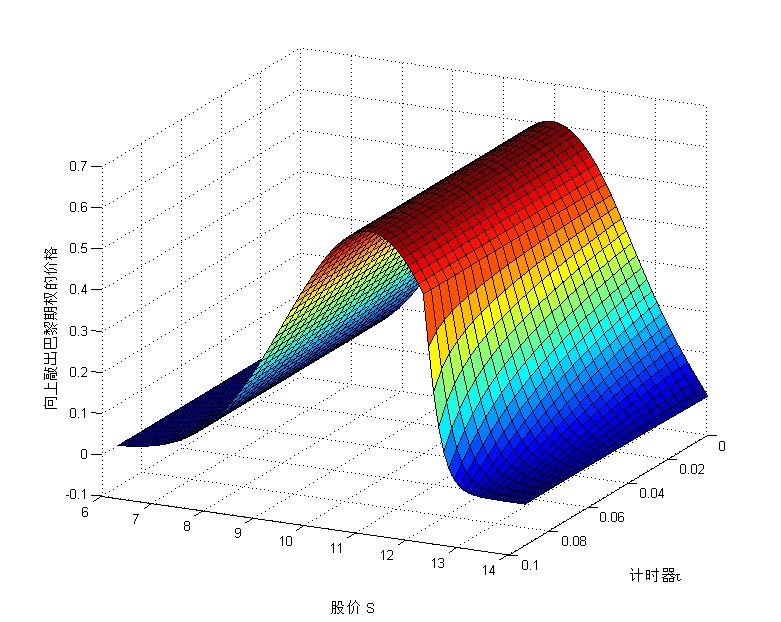
\includegraphics[width=8.5cm]{code/paris2.jpg}
\caption{连续型向上敲出看涨巴黎期权($t=0.5$)}
\end{minipage}
\begin{minipage}{0.48\linewidth}
\label{parisc2}
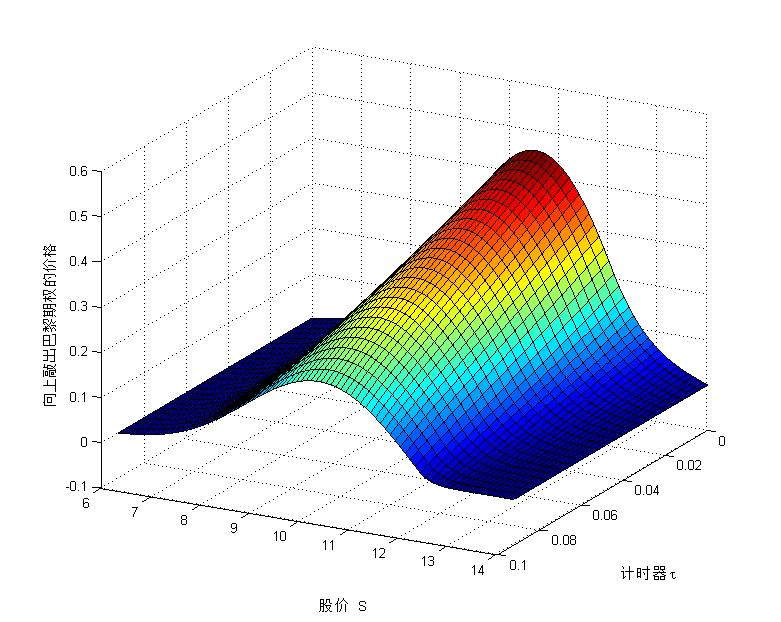
\includegraphics[width=8.5cm]{code/parisc2.jpg}
\caption{累计型向上敲出看涨巴黎期权($t=0.5$)}
\end{minipage}
\end{figure}
图\ref{paris2}为连续型向上敲出巴黎期权的价格,对于任何的参数$\tau$,最高点都约出现在$S=10.7$处,且峰值恒定。峰值左边对任何参数$\tau$,巴黎期权的价格只受股价参数$S$的影响。而峰值右边,巴黎期权的价格随着计时器$\tau$的增大而具有更快的下降速度。

图\ref{parisc2}为累计型向上敲出巴黎期权的价格,峰值会随着计时器$\tau$的增大而减小,并且稍稍向股价$S$减少的的方向便宜。整个函数图像会随着计时器$\tau$的增大而变得更平缓。对比连续型和累计型向上巴黎期权的价格,同样参数下,由于累计型巴黎期权中计时器不清零,因此其敲出的可能性更大,从而价格比连续型巴黎期权的价格更低。
\iffalse
\subsection{分数布朗运动}
布朗运动为分数布朗运动的当$H=0.5$的特殊情况。下面考虑当$W_t$为分数布朗运动时,不同参数$H$,对巴黎期权价格的影响。使用隐式差分法所得到的连续型和累计型向上敲出看涨巴黎期权价格分别为
\begin{figure}[H]
\begin{minipage}{0.48\linewidth}
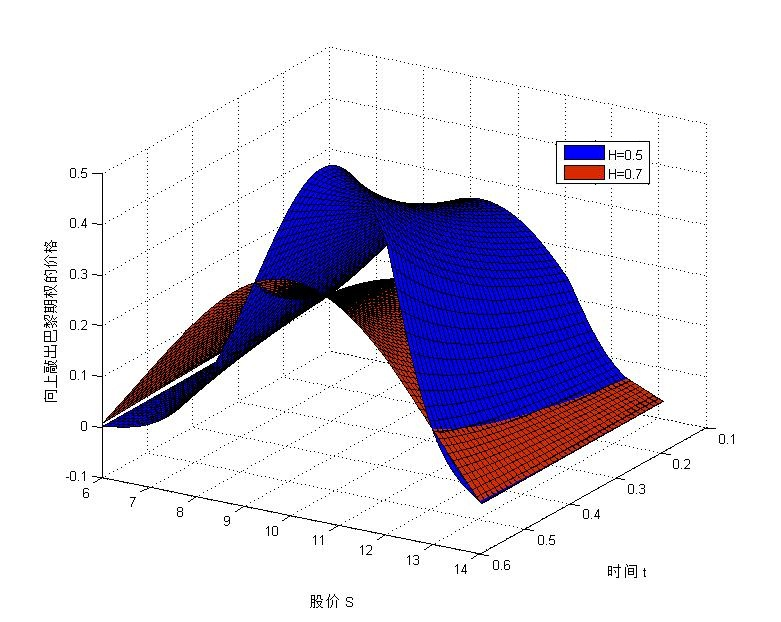
\includegraphics[width=8.5cm]{code/paris_fbm1.jpg}
\caption{连续型向上敲出看涨巴黎期权}
\end{minipage}
\begin{minipage}{0.48\linewidth}
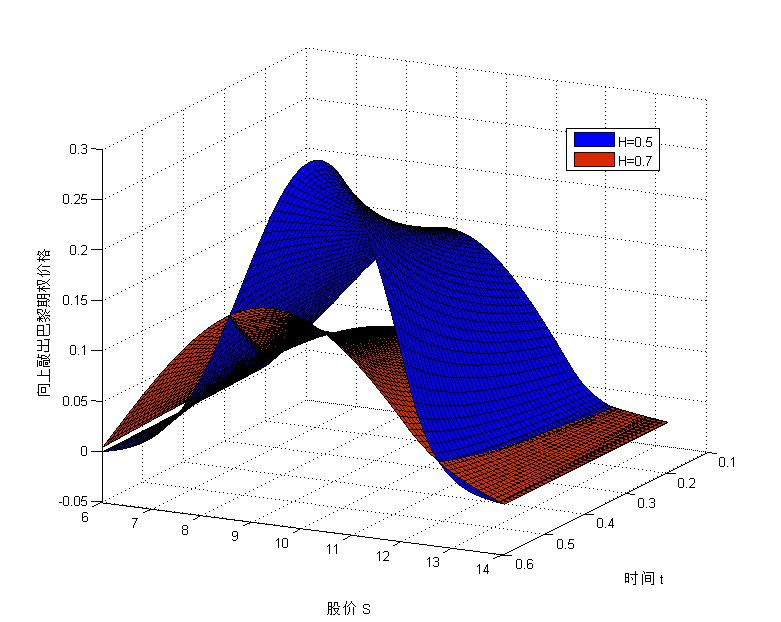
\includegraphics[width=8.5cm]{code/parisc_fbm1.jpg}
\caption{累计型向上敲出看涨巴黎期权}
\end{minipage}
\end{figure}
与布朗运动相比,在分数布朗运动的模型中,连续型与累计型巴黎期权的价格都有处明显的区别。首先表现为峰值下降并向左移动,其次是两侧曲面的下滑速度减满慢。

\begin{figure}[H]
\begin{minipage}{0.48\linewidth}
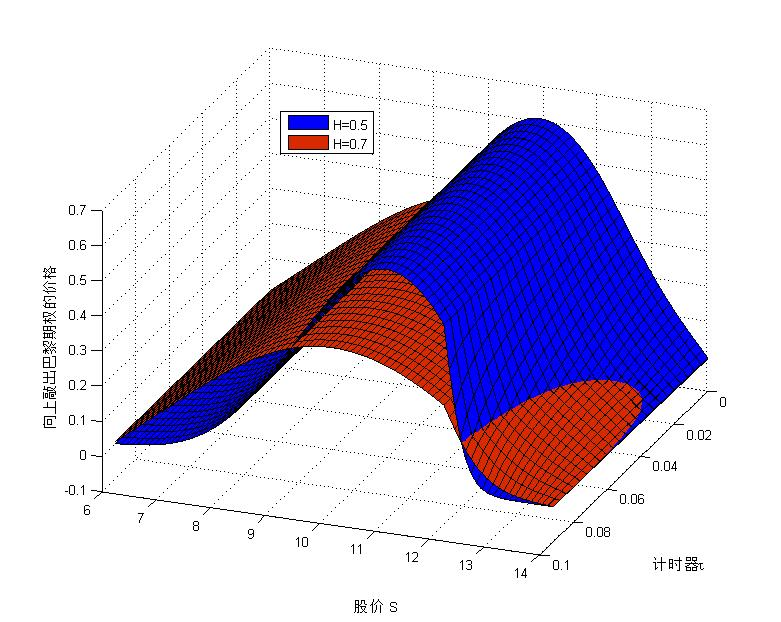
\includegraphics[width=8.5cm]{code/paris_fbm2.jpg}
\caption{连续型向上敲出看涨巴黎期权}
\end{minipage}
\begin{minipage}{0.48\linewidth}
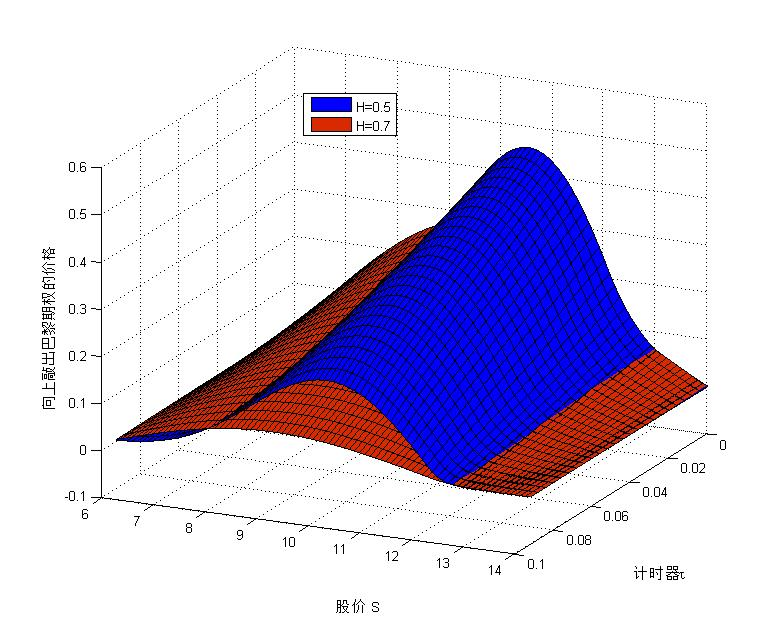
\includegraphics[width=8.5cm]{code/parisc_fbm2.jpg}
\caption{累计型向上敲出看涨巴黎期权}
\end{minipage}
\end{figure}
固定时间值$t$,同样能看到,相比布朗运动,分数布朗运动下巴黎期权价格的峰值向左移动,而相比连续型巴黎期权,累计型巴黎期权价格还随着计时器的增加而更快地减小。

考虑参数股价$S$在不同的参数$H$下对连续型向上敲出巴黎期权价格的影响
\begin{figure}[H]
\begin{center}
\label{paris_fbm}
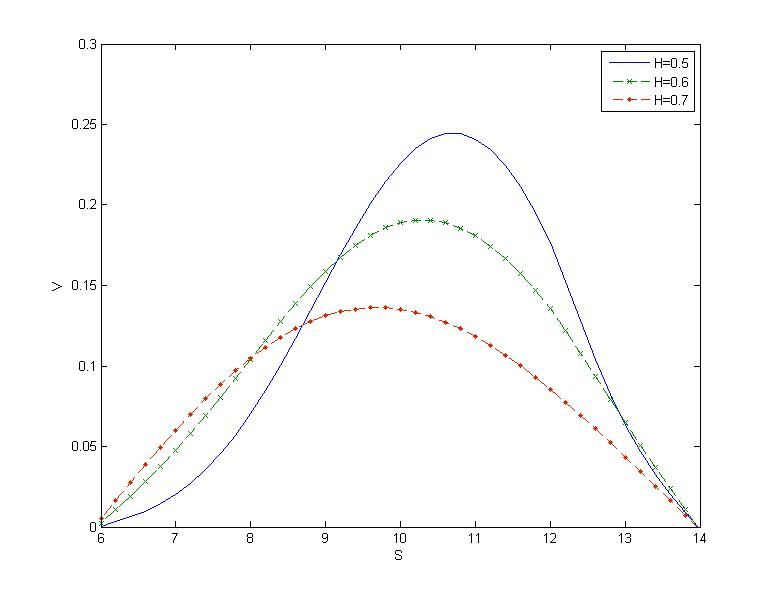
\includegraphics[width=10cm]{code/paris_fbm.jpg}
\caption{$S$与$V$的关系图}
\end{center}
\end{figure}
由图\ref{paris_fbm}可以看出,随着分数布朗运动的参数$H$的增加,标的资产的长期依赖性增强。股票的历史价格对股票未来走势的预测性增强,未来的不确定性减弱,整个巴黎期权价格的图像就会由陡峭逐渐变得肥胖。
\fi

\subsection{更广泛的高斯过程}
方程\eqref{hcon1}和\eqref{hcon2}可写成
\begin{equation}
-a^n_iV^{n}_{i-1}+(1-b^n_i)V^{n}_i-c^n_iV^{n}_{i+1}=V^{n+1}_i
\end{equation}
以及
\begin{equation}
-a^n_iV^{n}_{i-1,j}+(1-b^n_i)V^{n}_{i,j}-c^n_iV^{n}_{i+1,j}=V^{n+1}_{i,j+1}
\end{equation}
显然不同的高斯过程,影响计算结果的只有方程中的参数$U_n$,即方差函数的导数$U_t$。为了更一般性的研究不同的高斯过程对巴黎期权价格的影响,考虑表\ref{t1}中的三个不同的$U_t$函数(显然$U_3$即为参数$H=0.7$的分数布朗运动),研究不同的高斯过程对巴黎期权价格的影响。

\begin{table}[H]
\begin{minipage}{0.48\textwidth}
\caption{算例使用的协方差函数}
\centering
\label{t1}
\begin{tabular}{c|c|c|c|c}
\hline
 &$\alpha$&$\gamma$&$F_t$ & $U_t$ \\
\hline
$U_1$&$1$&$1$&$t$ & $1$ \\
$U_2$&$0.7$&$1$ & $0.7t$ & $0.7$ \\
$U_3$&$1.4$&$0.4$ & $t^{1.4}$ & $1.4t^{0.4}$ \\
\hline
\end{tabular}
\end{minipage}
\begin{minipage}{0.48\textwidth}
\centering
\begin{figure}[H]
\label{ut}
\centering
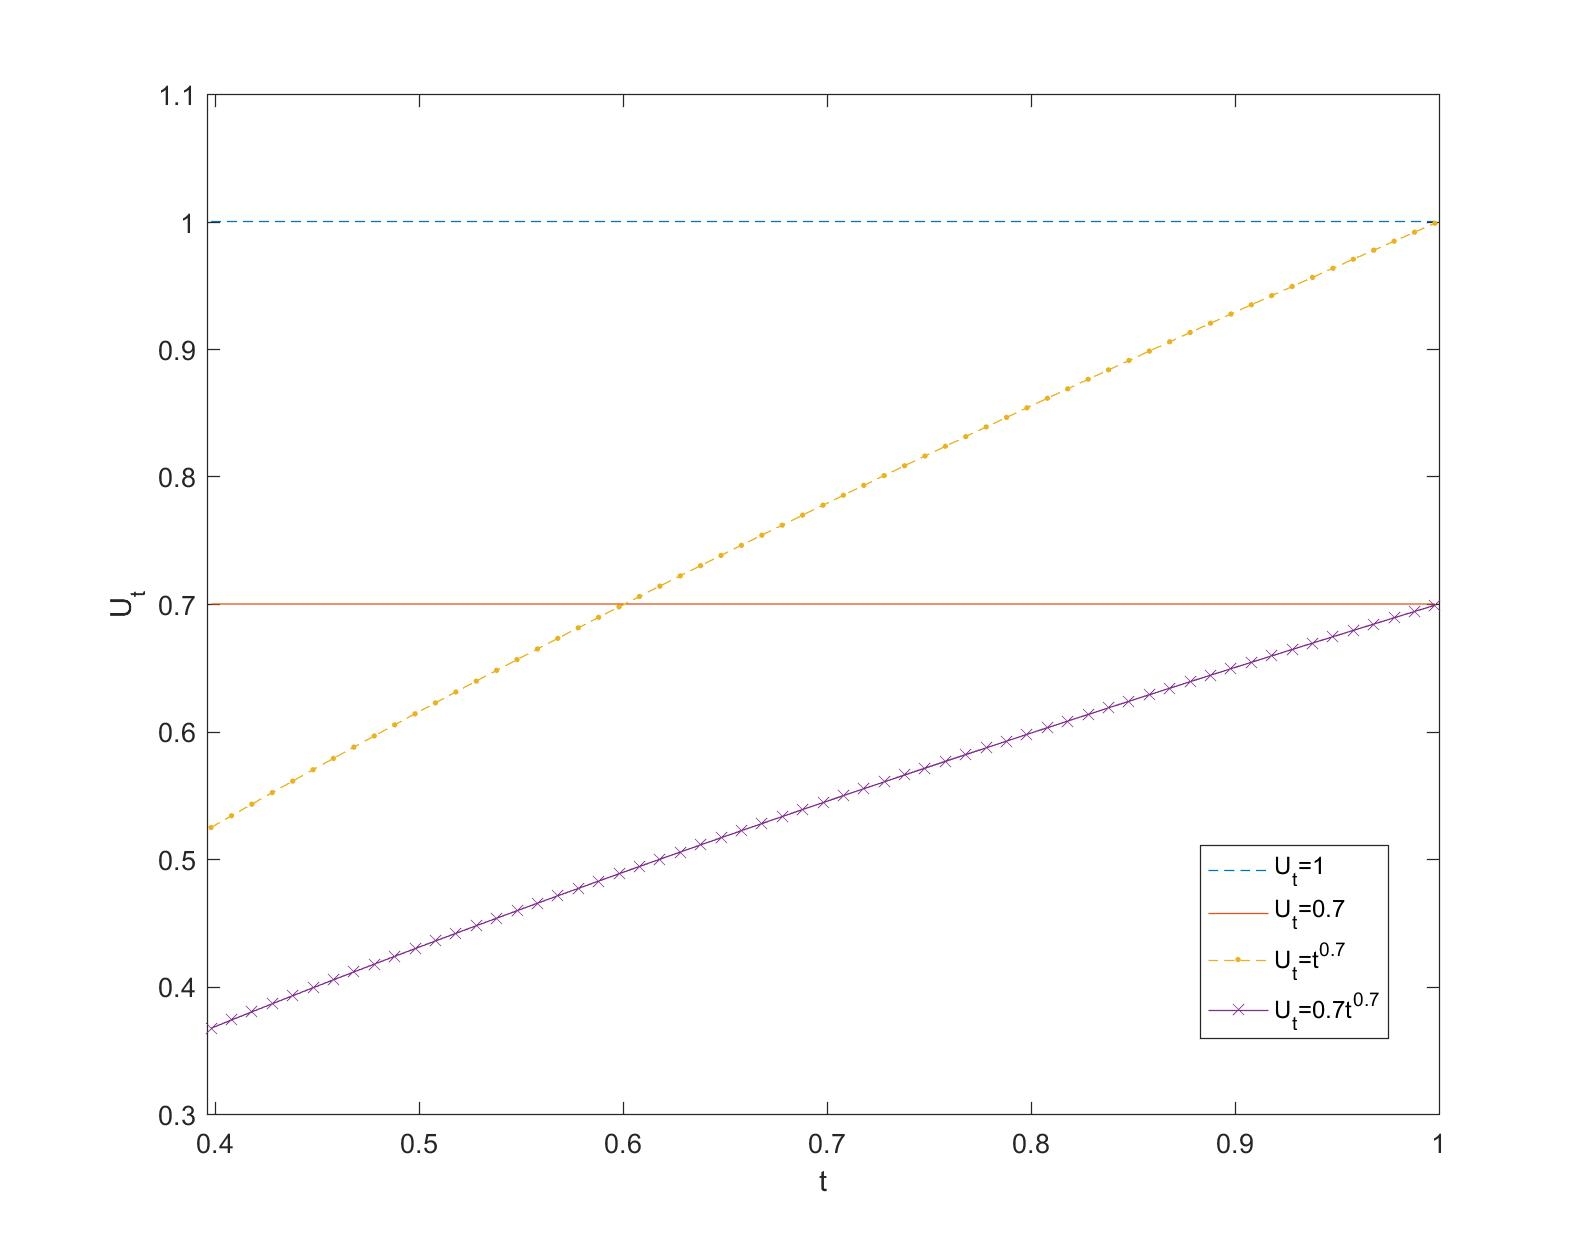
\includegraphics[width=8cm]{code/ut.jpg}
\caption{$U_t$的函数图}
\end{figure}
\end{minipage}
\end{table}

如图\ref{ut}所示,当$t>0.43$的时,有$U_2<U_1<U_3$;当$0.18<t<0.42$的时候,$U_2<U_3<U_1$;当$t<1.7$时,$U_3<U_2<U_1$。对不同的高斯过程,利用追赶法求解方程\eqref{hcon1}和\eqref{hcon2},以及方程组\eqref{hcmu},可分别得到的连续型和累计型向上敲出看涨巴黎期权价格,分别如图\ref{mg2}和图\ref{mc2}所示。显然,在固定的时间$t$下,不同的高斯过程影响了图像的陡峭程度。但类似的,连续型巴黎期权在不同的参数$\tau$下,峰值都出现在同一股价处。峰值左边只受股价$S$的影响,峰值右边会随着计时器$\tau$的增大而具有更快的下滑。同样参数下,累计型巴黎期权的价格更低。并且峰值会随着计时器$\tau$的增大而减小,并左移。函数图像会随着计时器$\tau$的增大而平缓。

\begin{figure}[H]
\label{mg2}
\begin{minipage}{0.48\linewidth}
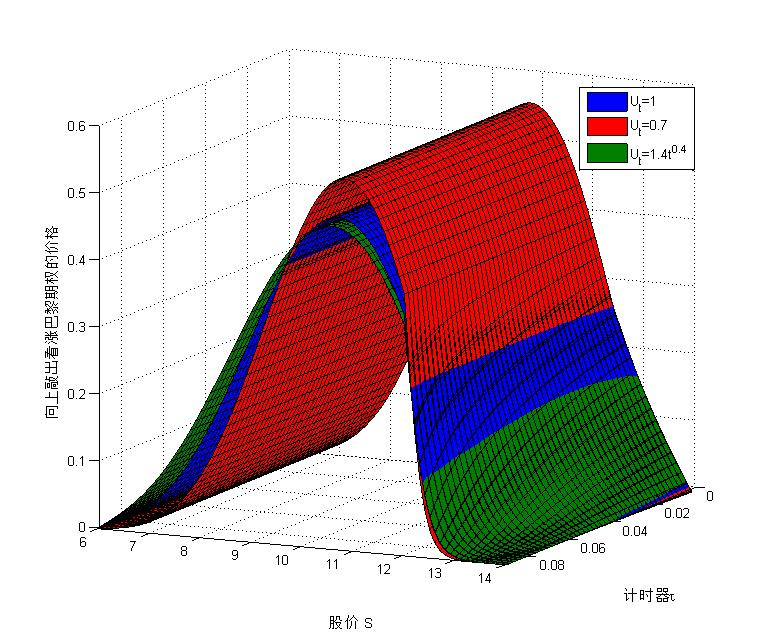
\includegraphics[width=8.5cm]{code/mg2.jpg}
\caption{连续型向上敲出看涨巴黎期权价格(t=0.5)}
\end{minipage}
\begin{minipage}{0.48\linewidth}
\label{mc2}
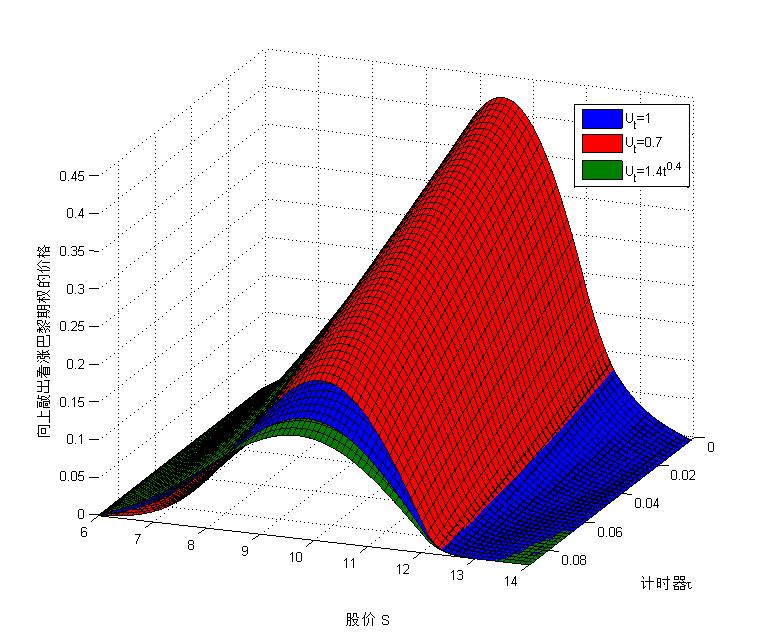
\includegraphics[width=8.5cm]{code/mc2.jpg}
\caption{累计型向上敲出看涨巴黎期权价格(t=0.5)}
\end{minipage}
\end{figure}

如图$t=0.5$,观察巴黎期权的图像\ref{mg2},显然不同参数$\alpha$,$\gamma$的高斯过程,
\begin{figure}[H]
\begin{minipage}{0.48\linewidth}
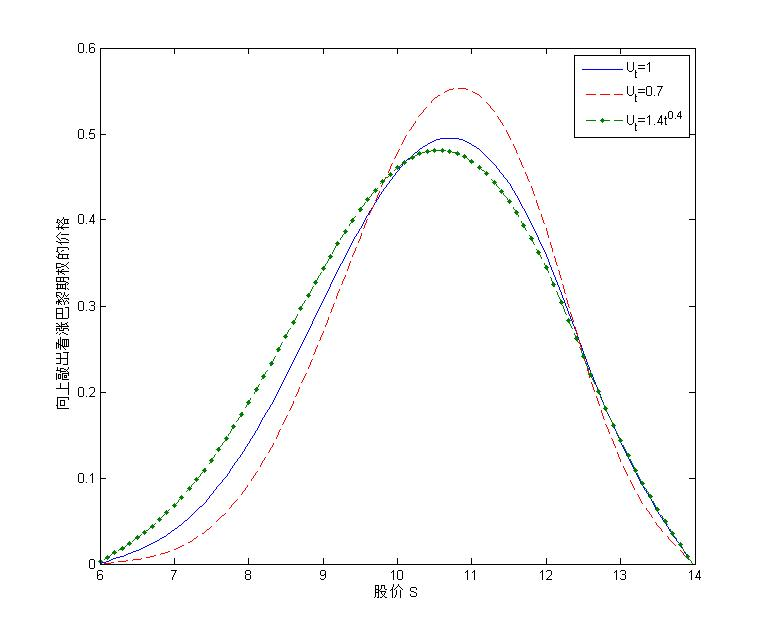
\includegraphics[width=8.5cm]{code/t0.5.jpg}
\caption{连续型巴黎期权的价格($t=0.5$,$\tau=0.01$)}
\end{minipage}
\begin{minipage}{0.48\linewidth}
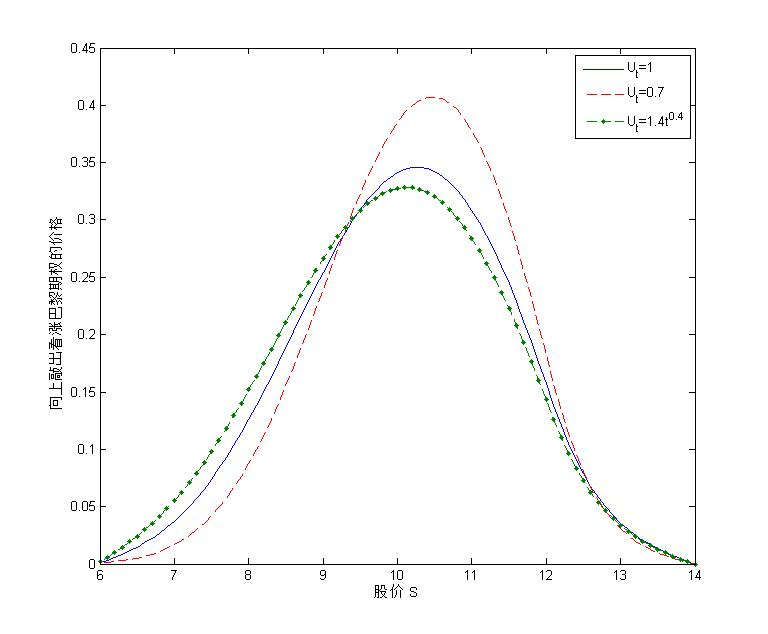
\includegraphics[width=8.5cm]{code/tc0.5.jpg}
\caption{累计型巴黎期权的价格($t=0.5$,$\tau=0.01$)}
\end{minipage}
\end{figure}

\begin{figure}[H]
\begin{minipage}{0.48\linewidth}
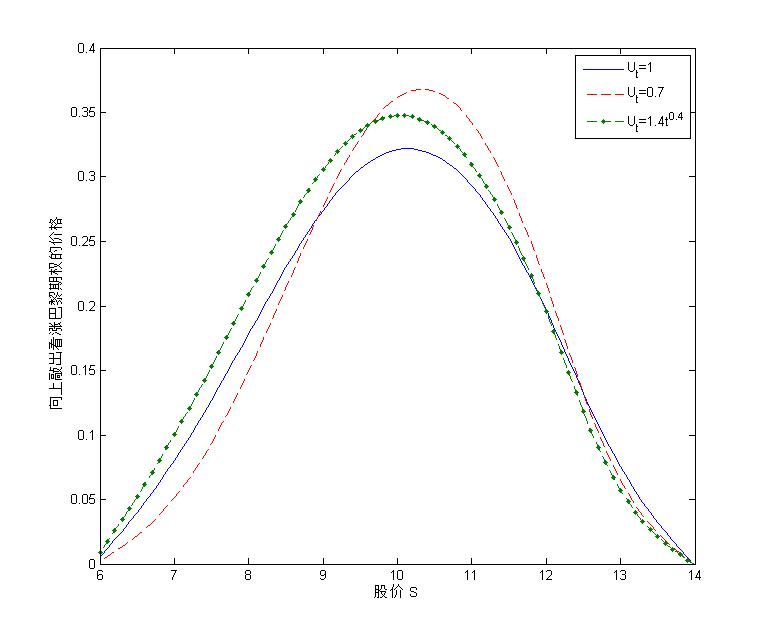
\includegraphics[width=8.5cm]{code/t0.2.jpg}
\caption{连续型巴黎期权的价格($t=0.2$,$\tau=0.01$)}
\end{minipage}
\begin{minipage}{0.48\linewidth}
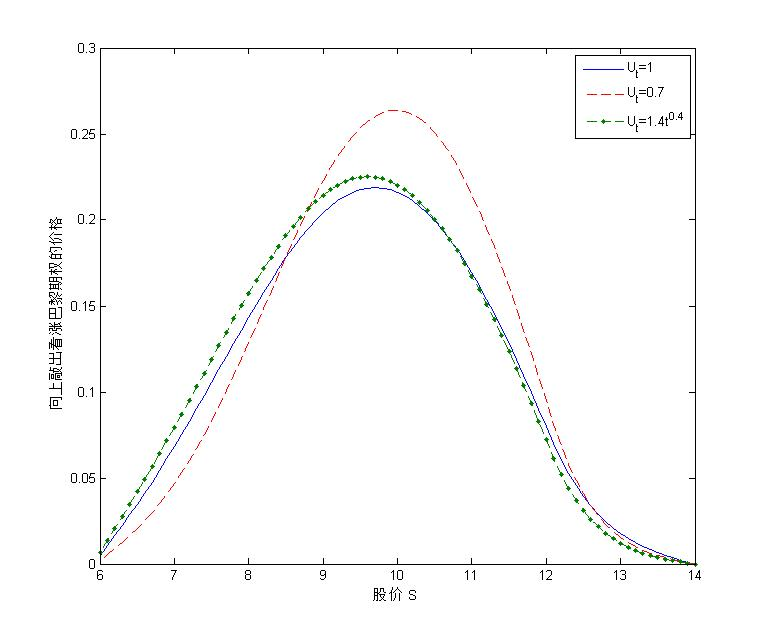
\includegraphics[width=8.5cm]{code/tc0.2.jpg}
\caption{累计型巴黎期权的价格($t=0.2$,$\tau=0.01$)}
\end{minipage}
\end{figure}

\begin{figure}[H]
\begin{minipage}{0.48\linewidth}
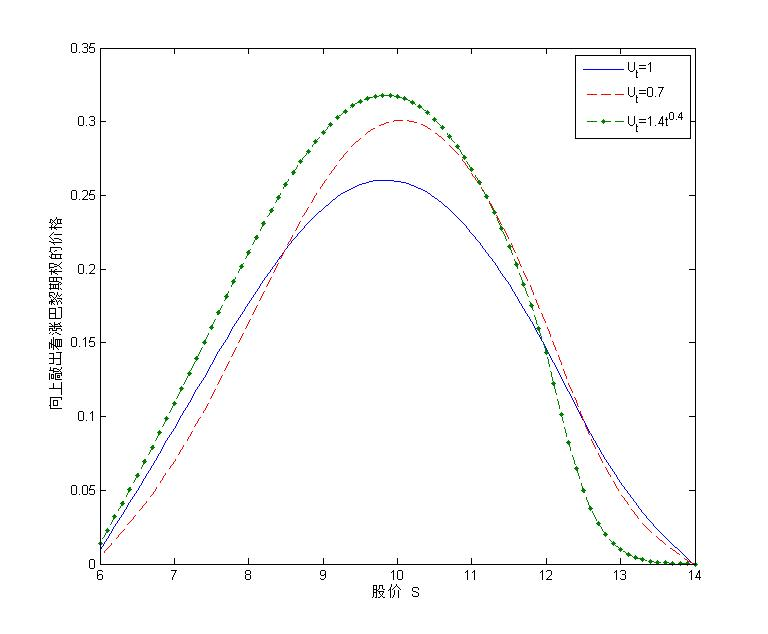
\includegraphics[width=8.5cm]{code/t0.jpg}
\caption{连续型巴黎期权的价格($t=0$,$\tau=0.01$)}
\end{minipage}
\begin{minipage}{0.48\linewidth}
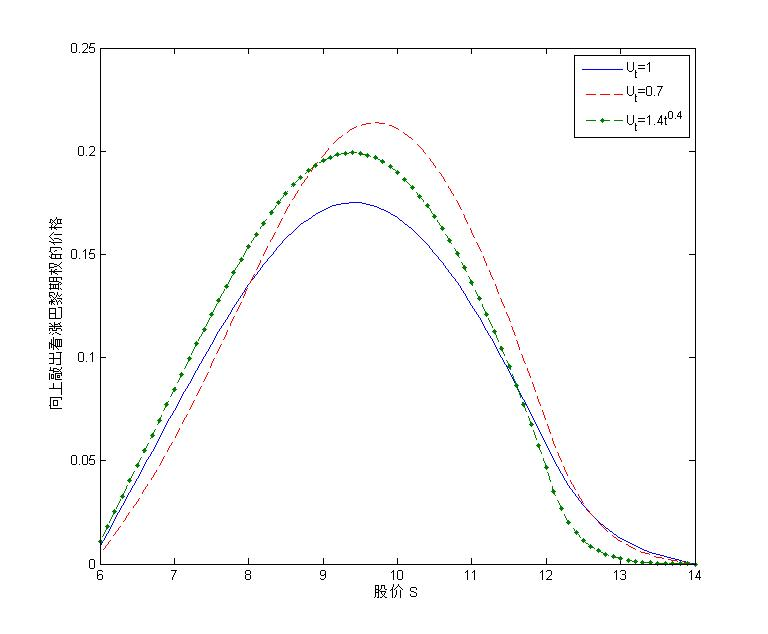
\includegraphics[width=8.5cm]{code/tc0.jpg}
\caption{累计型巴黎期权的价格($t=0$,$\tau=0.01$)}
\end{minipage}
\end{figure}

\section{结束语}
本文研究在一般高斯过程下连续型和累计型巴黎期权定价模型,并推导出一般高斯过程下巴黎期权价格的PDE。使用数值求解的方法,利用网格剖分,构造无条件稳定PDE的隐式差分格式,并使用计算量较小的追赶法进行求解。结果表明累计型巴黎期权的峰值明显低于连续型巴黎期权并且随着计时值$\tau$的增加而快速下降;分数和次分数布朗运动下,随参数$H$的增加,巴黎期权的峰值减少并向股价$S$减小的方向移动;(还没完) 


\begin{thebibliography}{10}
\bibitem{ref1}Chesney M, Cornwall J, Jeanblanc M, Kentwell G, Yor M. Parisian pricing [J]. Risk, 1997, 10(1): 77~79.
\bibitem{ref2}宋斌, 林则夫, 刘黎黎, 张冰洁. 基于博弈期权的可转债定价模型及其实证研究 [J]. 系统管理学报, 2013, 22(6): 758~767.
\bibitem{ref3}Haber J, Schonbucher J, Wilmott P. Pricing Parisian options [J]. The Journal of Theoretical and Applied Finance, 1999, 6(3): 71~79.
\bibitem{ref4}罗俊, 吴雄华. 巴黎期权定价问题的数值方法 [J]. 数值计算与计算机应用, 2004, 25(2): 81~89.
\bibitem{ref5}宋斌, 周湛满, 魏琳, 张冰洁. 巴黎期权的PDE定价及隐性差分法研究 [J]. 系统工程学报, 2013, 28(6): 764~774.
\bibitem{ref6}wok K, Lau W. Pricing algorithms for options with exotic path dependence [J]. Journal of Derivatives, 2001, 9(1): 28~38.
\bibitem{ref7}Longstaff F A, Schwartz E S. Valuing American options by simulation: A simple least-square approach [J]. Review of Financial Studies, 2001, 14(1): 113~147.
\bibitem{ref8}宋斌, 井帅. 美式巴黎期权的定价模型与数值方法 [J]. 系统工程, 2015, 33(2): 1~8.
\bibitem{ref9}wok K, Lau W. Pricing algorithms for options with exotic path dependence [J]. Journal of Derivatives, 2001, 9(1): 28~38.
\bibitem{ref10}Longstaff F A, Schwartz E S. Valuing American options by simulation: A simple least-square approach [J]. Review of Financial Studies, 2001, 14(1): 113~147.
\bibitem{ref11}宋斌, 井帅. 美式巴黎期权的定价模型与数值方法 [J]. 系统工程, 2015, 33(2): 1~8.
\bibitem{ref12} Rogers L. Arbitrage with fractional Brownian motion[J]. Mathematical Finance, 1997, 7(1): 95~105.
\bibitem{ref13} Nualart D, Taqqu M S. Wick-Ito formula for regular processes and applications to Black and Scholes formula [J]. Stochastics: An International Journal of Probability and Stochastic Processes, 2008, 80(5): 477~487.
\bibitem{ref14} Dai Q, Singleton, K J. Specification analysis of affine term structure models [J].Journal of Finance, 2000, 55(5): 1943~1978.
\bibitem{ref15} Peters E F. Fractal structure in the capital markets [J].Financial analyst Journal, 1989, 7(32): 434~453.
\bibitem{ref16} Hu Y, Øksendal B. Fractional white noise calculus and application to finance [J]. Infinite Dimensional Analysis, Quantum Probability and Related Topics, 2003, 1(6):1~32.
\bibitem{ref17}Lei P, Nualart D. A decomposition of the bi-fractional Brownian motion and some applications [J]. Statistics and Probability Letters, 2009, 79(5): 619~624.
\bibitem{ref18} Tudor C. Inner product spaces of integrands associated to sub-fractional Brownian motion [J]. Statistics and Probability Letters, 2008, 78(14): 2201~2209.
\bibitem{ref19} Zili M. On the mixed fractional Brownian motion[J]. Journal of Applied Mathematics and Stochastic Analysis, 2006, (32435):1~9.


\end{thebibliography}


\end{document}
